\documentclass[12pt,oneside]{uhthesis}
\usepackage{subfigure}
\usepackage[ruled,lined,linesnumbered,titlenumbered,algochapter,spanish,onelanguage]{algorithm2e}
\usepackage{amsmath}
\usepackage{amssymb}
\usepackage{amsbsy}
\usepackage{caption,booktabs}
\captionsetup{ justification = centering }
%\usepackage{mathpazo}
\usepackage{float}
\setlength{\marginparwidth}{2cm}
\usepackage{todonotes}
\usepackage{listings}
\usepackage{xcolor}
\usepackage{multicol}
\usepackage{graphicx}
\floatstyle{plaintop}
\restylefloat{table}
\sloppy
%\addbibresource{Bibliography.bib}
% \setlength{\parskip}{\baselineskip}%
\renewcommand{\tablename}{Tabla}
\renewcommand{\listalgorithmcfname}{Índice de Algoritmos}
%\dontprintsemicolon
\SetAlgoNoEnd
\bibliography{Bibliography}

\definecolor{codegreen}{rgb}{0,0.6,0}
\definecolor{codegray}{rgb}{0.5,0.5,0.5}
\definecolor{codepurple}{rgb}{0.58,0,0.82}
\definecolor{backcolour}{rgb}{0.95,0.95,0.92}
\definecolor{redstrings}{rgb}{0.9,0,0}
\lstdefinestyle{mystyle}{
	language=[Sharp]C,
    backgroundcolor=\color{white},   
%    commentstyle=\color{codegreen},
    keywordstyle=\color{blue},
    morekeywords={partial, var, value, get, set, T},
    numberstyle=\tiny\color{codegray},
    stringstyle=\color{redstrings},
%    basicstyle=\ttfamily\footnotesize,
    breakatwhitespace=true,         
    breaklines=true,                 
    captionpos=b,                    
    keepspaces=true,                 
    numbers=left,                    
    numbersep=5pt,                  
    showspaces=false,                
    showstringspaces=false,
    showtabs=false,                  
    tabsize=4,
%    
frame=lines,
escapeinside={(*@}{@*)},
commentstyle=\color{greencomments},
basicstyle=\ttfamily\small,
}

\lstset{style=mystyle}
\usepackage{spanish}

\title{Módulo fabric-chaincode-api para implementar contratos inteligentes empleando $C\sharp$.}
\author{\\\vspace{0.25cm}Amalia Nilda Ibarra Rodríguez}
\advisor{\\\vspace{0.25cm}Ing. Daniel Mena \\\vspace{0.25cm}Ing. Camilo  Denis González\\\vspace{0.2cm}Dr. Miguel Katrib Mora}
\degree{Licenciado en Ciencia de la Computación}
\faculty{Facultad de Matemática y Computación}
\date{Noviembre de 2022\\\vspace{0.25cm}\href{https://github.com/ic-matcom/fabric-chaincode-csharp}{github.com/ic-matcom/fabric-chaincode-csharp}}
\logo{Graphics/uhlogo}
\makenomenclature

\renewcommand{\vec}[1]{\boldsymbol{#1}}
\newcommand{\diff}[1]{\ensuremath{\mathrm{d}#1}}
\newcommand{\me}[1]{\mathrm{e}^{#1}}
\newcommand{\pf}{\mathfrak{p}}
\newcommand{\qf}{\mathfrak{q}}
%\newcommand{\kf}{\mathfrak{k}}
\newcommand{\kt}{\mathtt{k}}
\newcommand{\mf}{\mathfrak{m}}
\newcommand{\hf}{\mathfrak{h}}
\newcommand{\fac}{\mathrm{fac}}
\newcommand{\maxx}[1]{\max\left\{ #1 \right\} }
\newcommand{\minn}[1]{\min\left\{ #1 \right\} }
\newcommand{\lldpcf}{1.25}
\newcommand{\nnorm}[1]{\left\lvert #1 \right\rvert }
\renewcommand{\lstlistingname}{Ejemplo de código}
\renewcommand{\lstlistlistingname}{Ejemplos de código}

\begin{document}

\frontmatter
\maketitle

\begin{dedication}
A mis padres, por su apoyo en las tardes grises.\\
Porque para mi \textit{"nada es más grande que su amor"}. 
\end{dedication}
\begin{acknowledgements}
\begin{flushright}
\textit{A mis tutores Daniel, Camilo y Miguel Katrib.\\
A mi familia.\\
A mi novio Jose.\\
A mis amigos Gaby, Sandra, Ariel, Nadia, Luis y Jose.\\
A mis amigas Yosy, Susana y Ana Laura.\\
Gracias.}
\end{flushright}
\end{acknowledgements}
\begin{opinion}
El trabajo “Módulo fabric-chaincode-api para implementar contratos inteligentes empleando $C \sharp$”, desarrollado por la estudiante Amalia Ibarra Rodríguez, cumple con los requisitos para la culminación de la carrera de Ciencia de la Computación de la Universidad de La Habana.

El tema de investigación seleccionado es pertinente, oportuno y se enmarca dentro de las líneas de trabajo del grupo Blockchain del Instituto de Criptogafía de la Facultad de Matemática y Computación de la Universidad de La Habana que forman parte de un proyecto nacional de investigación.

Siendo Hyperledger Fabric (HLF) una de las plataformas usadas para el desarrollo de nuestras aplicaciones \textit{blockchain} y siendo $C \sharp$ uno de los lenguajes de programación más utilizados por la carrera y por la comunidad profesional, resulta conveniente desarrollar un módulo extensible que sirva de base para la implementación de contratos inteligentes para HLF usando el lenguaje $C \sharp$.

Para el desarrollo del trabajo la estudiante enfrentó el desafío en el poco tiempo disponible desde que se le planteó esta tarea. Ha tenido que asimilar en muy poco tiempo temas complejos como la tecnología \textit{blockchain} y en particular la plataforma empresarial HLF, lo cual tiene un valor adicional si lo valoramos en la culminación de un plan de estudios afectado por las dificultades generadas por la pandemia, la no presencialidad durante buena parte de la carrera y por no haber cursado estos temas en las asignaturas regulares.

La estudiante ha mostrado disciplina y dedicación en la realización del ejercicio, ha estado abierta a las críticas y señalamientos tanto en la redacción del trabajo de diploma, como en la organización y la implementación de la solución mostrando buenas capacidades de investigación y de programación.

Por su propia naturaleza y complejidad el trabajo requiere de continuidad en cuanto a su prueba y ampliación por lo que esperamos que la diplomante, una vez graduada, esté abierta a la cooperación posterior con nuestro colectivo para mejorar los aspectos que se le puedan señalar durante el proceso de defensa y discusión de su trabajo.
 
Consideramos que tanto el \textit{software} desarrollado como el documento escrito, si bien siempre susceptibles de mejora, tienen el rigor metodológico y científico adecuado y está en función de los requisitos planteados.

Por tanto, felicitamos a la estudiante y consideramos que la tesis reúne los estándares metodológicos exigidos por la Facultad de Matemática y Computación de la Universidad de la Habana, para ser presentada y sometida a evaluación en su ejercicio de defensa.

La Habana, Diciembre 7 de 2022\\

Daniel Frías Mena $\_\_\_\_\_\_\_\_\_\_\_\_\_\_\_$\\

Camilo Denis González $\_\_\_\_\_\_\_\_\_\_\_\_\_\_\_$\\

Miguel Katrib Mora $\_\_\_\_\_\_\_\_\_\_\_\_\_\_\_$\\

\end{opinion}
\begin{resumen}
Hyperledger Fabric es una plataforma de tecnología de libro mayor distribuido de código abierto, diseñada para su uso en contextos empresariales.

Una característica que distingue Hyperledger Fabric de otras \textit{blockchains} es su capacidad de admitir contratos inteligentes escritos en lenguajes de programación de propósito general. Actualmente Go, Java y Node.js son los lenguajes soportados.

En este trabajo se presenta la herramienta \texttt{fabric-chaincode-csharp}, una biblioteca que permite el desarrollo de contratos inteligentes en $ C\sharp $.
\end{resumen}

\begin{abstract}
Hyperledger Fabric is an open source enterprise-grade permissioned distributed ledger technology platform, designed for use in enterprise contexts.

One feature that sets Hyperledger Fabric apart from other blockchains is its ability to admit smart contracts authored in general-purpose programming languages. Currently Go, Java and Node.js are supported.

This paper presents the \texttt{fabric-chaincode-csharp} tool, a library which allows the development of smart contracts in $ C\sharp $.
\end{abstract}
\include{FrontMatter/Contents}

\mainmatter

\chapter*{Introducción}\label{chapter:introduction}
\addcontentsline{toc}{chapter}{Introducción}

Hyperledger Fabric es una plataforma de tecnología de libro mayor distribuido (DLT) de código abierto, diseñada para su uso en contextos empresariales [\cite{hlf-doc}]. Su arquitectura altamente modular y configurable permite la innovación, la versatilidad y la optimización para una amplia gama de casos de uso de la industria, incluidos la banca, las finanzas, los seguros, la atención médica, los recursos humanos, la cadena de suministro e incluso la entrega de música digital.

Entre las capacidades que distinguen a Hyperledger Fabric de otras blockchains destaca ser la primera plataforma DLT que admite contratos inteligentes creados en lenguajes de programación de propósito general como Java, Go y Node.js.
Esto significa que la mayoría de las empresas no necesitan capacitación adicional para aprender un nuevo idioma o DSL para poder trabajar con Hyperledger Fabric, por tanto, es una ventaja.

Para lograr esta capacidad, Hyperledger Fabric implementa una arquitectura para las transacciones llamada \textit{execute-order-validate} [\cite{hlf-paper}], que permite eliminar el no determinismo en los contratos inteligentes independientemente del lenguaje en el que se programen. Como consecuencia, la lista de lenguajes mencionada anteriormente puede ser extensible a cualquier otro lenguaje de programación. 


%Los contratos inteligentes que se ejecutan en una Blockchain deben ser deterministas; de lo contrario, es posible que nunca se llegue a un consenso. Para abordar el problema del no determinismo, muchas plataformas requieren que los contratos inteligentes se escriban en un lenguaje específico de dominio restringido (como Solidity) para que se puedan eliminar las operaciones no deterministas.

%En Fabric, una política de respaldo específica de la aplicación especifica qué nodos pares, o cuántos de ellos, deben garantizar la ejecución correcta de un contrato inteligente determinado. Por lo tanto, cada transacción solo necesita ser ejecutada (aprobada) por el subconjunto de los nodos pares necesarios para satisfacer la política de aprobación de la transacción. Esto permite una ejecución paralela que aumenta el rendimiento general y la escala del sistema. Esta primera fase también elimina cualquier no determinismo, ya que los resultados inconsistentes se pueden filtrar antes de realizar el pedido.

%Debido a que eliminamos el no determinismo, Fabric es la primera tecnología de cadena de bloques que permite el uso de lenguajes de programación estándar.

A partir de esta posibilidad el Instituto de Criptografía de la Universidad de la Habana, ante la necesidad existente de poder utilizar lenguajes de propósito general para el desarrollo de los contratos con Hyperledger Fabric, traza como    \textbf{objetivo general} integrar la lógica de los contratos inteligentes programados en $C\sharp$ dentro de la arquitectura de una blockchain Hyperledger Fabric.

%El lenguaje $C \sharp$ es un requerimiento del Instituto? Bueno, además de contar con una amplia comunidad de desarrolladores alrededor del mundo $C \sharp$ es el lenguaje con el que los estudiantes de la carrera de Ciencias de la Computación aprenden a programar. Poder crear contratos inteligentes en un lenguaje conocido es una ventaja que incentiva el acercamiento al mundo del Blockchain en los primeros años de la carrera.

El \textbf{problema a resolver} consiste entonces en crear las condiciones técnicas y documentación con el fin de garantizar la programación de contratos inteligentes para Hyperledger Fabric  escritos en $C\sharp$.

Se propone construir una API fabric-contract-api-csharp,  que proporcione la interfaz del contrato, un punto de entrada de alto nivel para escribir la lógica empresarial.

Para el cumplimiento de este objetivo general se llevarán a cabo las \textbf{siguientes tareas}:

\begin{enumerate}
\item Estudio de las APIs existentes para los lenguajes actualmente soportados.
\item Diseño e implementación del Software Development Kit (SDK).
\item Desarrollo de un repositorio de contratos reutilizables.
\end{enumerate}

\subsection*{Presentación de los siguientes capítulos}	

\chapter{Estado del Arte}\label{chapter:state-of-the-art}


\colorbox{lightgray}{\textbf{//TODO: Presentacion del capitulo: qué se va a tratar y por qué}}

\section{Qué es una Blockchain}
En esencia, una blockchain es un \textbf{\textit{ledger}} distribuido que registra todas las transacciones que tienen lugar en la red. El \textit{ledger} de una \textit{blockchain} a menudo se describe como descentralizado porque se replica entre muchos participantes de la red, cada uno de los cuales colabora en su mantenimiento.

La información registrada en una \textit{blockchain}, además de ser \textbf{descentralizada} y \textbf{colaborativa}, sólo se puede agregar. Esto significa que se garantiza, utilizando técnicas criptográficas, que una vez  agregada una transacción al \textit{ledger}, no se puede modificar. Esta propiedad de inmutabilidad simplifica la determinación de la procedencia de la información pues los participantes pueden estar seguros de que esta no ha cambiado después de añadirse a la \textit{blockchain}.

Con el fin de respaldar la actualización constante de la información, y  habilitar una gran cantidad de funciones del \textit{ledger} (transacciones, consultas, etc.), una red  blockchain utiliza \textbf{contratos inteligentes}. Estos constituyen una forma de proporcionar acceso controlado al \textit{ledger}.

Una red  \textit{blockchain} se compone principalmente de un conjunto de \textbf{nodos \textit{peers}} (o simplemente \textit{peers}). Dichos nodos son un elemento fundamental de la red debido a que alojan \textit{ledgers} y contratos inteligentes.

Se le llama \textbf{consenso} al proceso de mantener las transacciones sincronizadas a través de la red con el objetivo de garantizar que los \textit{ledgers} se actualicen solo cuando las transacciones sean aprobadas por los participantes apropiados; y con las transacciones en el mismo orden.

\section{Hyperledger Fabric}

Hyperledger Fabric, o simplemente Fabric, es uno de los proyectos de blockchain dentro de Hyperledger [\cite{hyperledger-foundation}], auspiciado por la Fundación Linux [\cite{linux-foundation}]. Es una plataforma de \textbf{tecnología de \textit{ledger} distribuido} (DLT por sus siglas en inglés) de código abierto, diseñada para su uso en contextos empresariales. Además, se define como una red permisionada, lo que significa que los participantes se conocen entre sí, en lugar de ser anónimos. 

Al igual que otras tecnologías \textit{blockchain}, Hyperledger Fabric cuenta con un \textit{\textbf{ledger}}, utiliza \textbf{contratos inteligentes} y es un sistema mediante el cual los participantes realizan sus \textbf{transacciones}.

Las redes de Hyperledger Fabric son administradas por una colección de \textbf{organizaciones}. Los nodos \textit{\textbf{peer}} son fundamentales para construir este tipo de red distribuida porque son propiedad de estas organizaciones y sus puntos de conexión a la red. 

Al ser una plataforma permisionada, Hyperledger Fabric permite la confidencialidad a través \textbf{canales}. En estos, los participantes establecen una \textit{sub-red} donde cada miembro tiene visibilidad de un conjunto particular de transacciones. Así, solo aquellos nodos que participan en un canal tienen acceso al contrato inteligente y a los datos transados, preservando la privacidad y confidencialidad de ambos.
Esta es una opción especialmente importante para las redes en las que algunos participantes pueden ser competidores y no quieren que cada transacción sea conocida por el resto de la red. 

%Fabric es la primera plataforma DLT que admite \textbf{contratos inteligentes} creados en lenguajes de programación de propósito general como Java, Go y Node.js, en lugar de lenguajes específicos de dominio restringidos (DSL).

\subsection*{Ledger}

El \textit{ledger} de Hyperledger Fabric consta de dos componentes: el \textbf{world state} y el \textbf{registro de transacciones}. Cada participante tiene una copia del \textit{ledger} de cada red de Hyperledger Fabric a la que pertenece.

El componente de \textit{world state} describe el estado del \textit{ledger} en un momento determinado, es la base de datos del mismo. El componente de registro de transacciones almacena todas las transacciones que dieron como resultado el valor actual del \textit{world state}. Es el historial de actualizaciones del \textit{world state}. El \textit{ledger}, entonces, es una combinación de la base de datos del \textit{world state} y el historial del registro de transacciones.

\subsection*{Contratos inteligentes}

Los desarrolladores de aplicaciones de cada organización pueden crear \textbf{contratos inteligentes }para implementar un proceso comercial compartido por los miembros del consorcio. Los contratos inteligentes se utilizan para ayudar a generar \textbf{transacciones} que luego se pueden distribuir a cada nodo de la red.

Los contratos inteligentes de Hyperledger Fabric se definen dentro del \textbf{\textit{chaincode}}. Se pueden definir múltiples contratos inteligentes dentro del mismo \textit{chaincode}. Cuando este despliega, todos los contratos inteligentes dentro de él se hacen disponibles para las aplicaciones externas a la \textit{blockchain}. Una aplicación  invoca al contrato inteligente cuando esta necesita interactuar con el \textit{ledger}. 

En la mayoría de los casos, el \textit{chaincode} interactúa sólo con el componente de la base de datos del ledger, el \textbf{\textit{world state}} (consultándolo, por ejemplo) y no con el registro de transacciones.

Los usuarios de Hyperledger Fabric a menudo usan los términos \textbf{contrato inteligente} y \textbf{\textit{chaincode}} indistintamente. En general, un contrato inteligente define la lógica de transacción que controla el ciclo de vida de un objeto contenido en el \textit{world state}; luego, este se empaqueta en un \textit{chaincode} para desplegarse a una red \textit{blockchain}.

\subsection*{Consenso}
Las transacciones deben escribirse en el ledger en el orden en que ocurren, aunque puedan ser entre diferentes conjuntos de participantes dentro de la red. Para que esto suceda, se debe establecer el orden de las transacciones y se debe implementar un método para rechazar transacciones incorrectas que se hayan insertado en el ledger por error (o maliciosamente).

Los \textit{peers} ejecutan un \textbf{protocolo de consenso} que abarca desde la propuesta y la aprobación de transacciones hasta el orden, la validación y el despliegue de las mismas a través de la red.
En pocas palabras, el \textbf{consenso} se define como la verificación completa de la correctitud de un conjunto de transacciones que componen un bloque [\cite{hlf-doc}].

El consenso está mediado por nodos especiales llamados \textit{\textbf{orderers}}, encargados de ordenar las transacciones. Un conjunto de nodos \textit{orderers} forman un \textbf{\textit{ordering service}}. Además de su rol de ordenar, estos nodos también mantienen la lista de organizaciones que pueden crear canales. Esta lista se conoce como el \textbf{consorcio}.

%Sin embargo, el consenso abarca más que simplemente acordar el orden de las transacciones, y esta diferenciación se destaca en Hyperledger Fabric a través de su papel fundamental en todo el flujo de transacciones, desde la propuesta y el respaldo hasta el pedido, la validación y el compromiso. 

\begin{figure}[tbph]
\centering
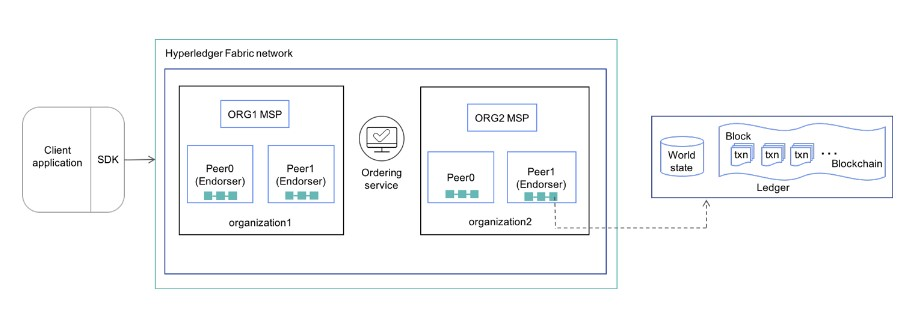
\includegraphics[width=\textwidth]{Images/hlf_components}
\caption{Componentes de Hyperledger Fabric}
\label{fig:hlfcomponents}
\end{figure}


\subsection*{Arquitectura para las transacciones \textit{execute-order-validate}.}

Fabric admite el uso de lenguajes de programación estándar en sus contratos inteligentes. Esto gracias a que implementa la arquitectura de ejecución de transacciones \textit{execute-order-validate}.

%Para entender por qué es posible añadir $C\sharp$ a la lista de lenguajes soportados por Hyperledger Fabric para programar contratos inteligentes, se dedicará esta sección a explicar dicha arquitectura.

Todos los sistemas de blockchains anteriores a Hyperledger Fabric, autorizados o no, siguen la arquitectura de ejecución de transacciones \textit{order-execute} [\cite{hlf-paper}]. Esto significa que la red blockchain ordena las transacciones primero, utilizando un protocolo de consenso, y luego los ejecuta en el mismo orden en todos los nodos \textit{peer} secuencialmente.

%La arquitectura \textit{order-execute} es conceptualmente simple y por lo tanto también muy utilizada. Sin embargo, tiene varios inconvenientes cuando se implementa en una blockchain autorizada de uso general.

Un problema importante para una arquitectura \textit{order-execute} son las transacciones no deterministas. Las operaciones que se ejecutan después del consenso deben ser deterministas, o el \textit{ledger} distribuido se “bifurca” y viola la premisa básica de una blockchain, que todos los nodos \textit{peer} tienen el mismo estado. Esto generalmente se aborda mediante la programación de \textit{blockchains} en un DSL (ej. Ethereum Solidity) que son lo suficientemente expresivos para sus aplicaciones pero limitados a una ejecución determinista.

Dichos lenguajes son difíciles de diseñar y requieren
aprendizaje adicional por parte del programador. La redacción de contratos inteligentes en un lenguaje de propósito general (p. ej., Go, Java, C/C++) parece más atractivo y acelera la adopción de soluciones blockchain.

%Desafortunadamente, los lenguajes de propósito general plantean muchos problemas para garantizar una ejecución determinista. Incluso si el desarrollador de la aplicación no introduce operaciones obviamente no deterministas, detalles ocultos de implementación pueden tener el mismo efecto devastador (por ejemplo, un
%iterador de mapa no es determinista en Go).

Fabric introduce la arquitectura de ejecución de transacciones \textit{order-execute-validate} y no sigue el diseño \textit{order-execute} estándar. Aborda los desafíos de resiliencia, flexibilidad, escalabilidad, rendimiento y confidencialidad que enfrenta el modelo \textit{order-execute} al separar el flujo de transacciones en tres pasos:
\begin{enumerate}
 \item \textbf{ejecutar} una transacción y verificar su correctitud, avalándola.
 \item \textbf{ordenar} transacciones a través de un protocolo de consenso.
   \item \textbf{validar} transacciones contra una política de aprobación específica de la aplicación antes de actualizar el \textit{ledger}.
\end{enumerate}

Este diseño se aparta del paradigma \textit{order-execute} en el sentido de que Fabric ejecuta transacciones antes de llegar a un acuerdo final sobre su orden. De esta forma se elimina cualquier no determinismo, ya que los resultados inconsistentes se pueden filtrar antes de ordenar.

Al eliminar el no determinismo, Fabric es la primera blockchain que permite el uso de lenguajes de programación estándar. 

%Gracias a esta posibilidad, en este trabajo se pretende añadir $C\sharp$ a la lista de lenguajes actualmente soportados.

%\subsection*{Flujo de una transacción}
%El flujo de solicitud de alto nivel de una transacción en una red de Hyperledger Fabric es así:
%
%\begin{enumerate}
%\item El cliente se conecta a una red de Hyperledger Fabric mediante Node.js o Java™ SDK. Usando la API SDK, el cliente crea una transacción y la envía al par que la respalda.
%
%\item El par que respalda verifica la firma del cliente, simula una transacción y envía una firma de respaldo.
%
%\item Si la transacción está endosada, el cliente envía la transacción al servicio de pedidos. De lo contrario, la transacción se cancela.
%
%\item El servicio de pedidos entrega una transacción a los pares. Todos los pares comprometen y aplican la misma secuencia de transacciones y actualizan su estado.
%\end{enumerate}

\begin{figure}[tbph]
\centering
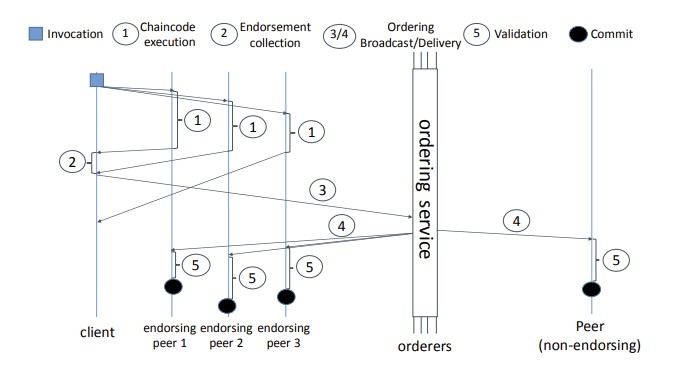
\includegraphics[width=\textwidth]{Images/transaction_flow}
\caption{Flujo de una transacción}
\label{fig:transactionflow}
\end{figure}



%Los lenguajes actualmente soportados son Java, Go y Node.js.
%Para entender cómo es posible añadir otro lenguaje para implementar contratos inteligentes, se hará énfasis en la fase de ejecución, donde el chaincode y el nodo peer se comunican. 

%\section{Fase de ejecución}
%
%En la fase de ejecución, los clientes firman y envían la propuesta de transacción a uno o más nodos \textit{peers} para su ejecución.  La propuesta es una solicitud para invocar una función del \textit{chaincode} con ciertos parámetros de entrada, con la intención de leer y/o actualizar el \textit{ledger}. Una aplicación que aprovecha un SDK compatible (Node, Java, Go) utiliza una de las API disponibles para generar una propuesta de transacción.
%
%El SDK sirve como un \textit{shim} para empaquetar la propuesta de transacción en el formato diseñado correctamente (\textit{protocol buffer} sobre gRPC) y toma las credenciales criptográficas del usuario para producir una firma única para esta propuesta de transacción. 



\section{fabric-contract-apis y fabric-chaincode-apis}
Hyperledger Fabric ofrece una serie de APIs para respaldar el desarrollo de contratos inteligentes (\textit{chaincode}) en varios lenguajes de programación (Go, Java y Node.js). 

Las \textit{fabric-chaincode-apis} son responsables de ejecutar el contrato inteligente, hacerlo accesible para el nodo \textit{peer} y administrar toda la interacción de bajo nivel con él a través de gRPC. Además, proporcionan la interfaz  \texttt{Chaincode} al contrato inteligente para acceder a los servicios de invocación del \textit{ledger} y el \textit{chaincode} mediante el \textit{chaincode stub} [\cite{hlf-internals}].

Las \textit{fabric-contract-apis} importan las bibliotecas \textit{fabric-chaincode-apis }y  proveen la interfaz \texttt{Contract}. Esta constituye un punto de entrada de alto nivel que permite abstraer al desarrollador de procedimientos de configuración de la red y concentrarse en implementar la lógica empresarial.
%
%Ambas bibliotecas propician al desarrollador las herramientas necesarias para implementar contratos inteligentes. En los lenguajes Java y Node.js las fabric-chaincode-apis conforman un módulo dentro de la biblioteca fabric-contract-api. En Go implementa la fabric-chaincode-api 
 
El módulo chaincode shim, o simplemente shim, constituye el componente principal de las fabric-chaincode-apis. En esta sección se aborda la implementación del \textit{chaincode shim} en la biblioteca \textit{fabric-chaincode-go}. Se analiza la arquitectura, el diseño, sus componentes clave y el protocolo utilizado para interactuar con el \textit{peer}.

%Un contrato inteligente se define dentro de un chaincode. Se pueden definir múltiples contratos inteligentes dentro del mismo chaincode. Cuando se implementa un chaincode, todos los contratos inteligentes dentro de él se ponen a disposición de las aplicaciones.

%La siguiente figura proporciona una descripción general de los componentes principales que están involucrados en la interacción entre el proceso del chaincode y el \textit{peer}.
%
%\begin{figure}[tbph]
%\centering
%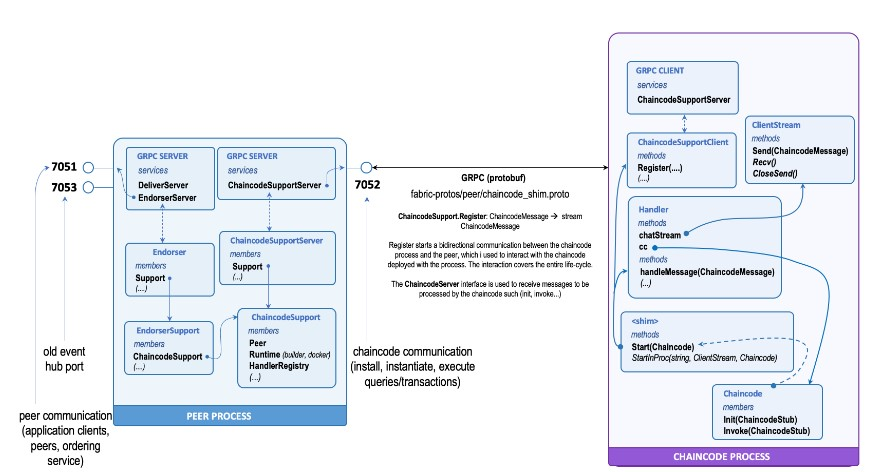
\includegraphics[width=\textwidth]{Images/peer_chaincode_interaction}
%\caption{}
%\label{fig:peerchaincodeinteraction}
%\end{figure}



\subsection*{Chaincode shim}

Con el fin de simplificar la vida del desarrollador y centrar sus esfuerzos en implementar la lógica del contrato inteligente, Hyperledger proporciona los \textit{chaincode shims}. Se trata de la implementación del \textit{runtime environment} necesario para integrar el contrato inteligente con Hyperledger Fabric y ejecutarlos como procesos remotos.

%El \textit{shim} es el componente responsable de ejecutar el contrato inteligente, hacerlo accesible para el nodo \textit{peer} y administrar toda la interacción de bajo nivel con él a través de gRPC. Además, proporciona una interfaz simplificada para el contrato inteligente para acceder a los servicios de invocación del \textit{ledger} y el \textit{chaincode} a través del \textit{chaincode stub} [\cite{hlf-internals}].

La figura \ref{fig:chaincodeshim} proporciona un desglose de los componentes que conforman el proceso chaincode junto con el rol y las responsabilidades que tiene cada uno de los componentes. Vale la pena señalar que, si bien el \textit{shim} es un componente específico del proceso chaincode, a menos que se especifique lo contrario, el \textit{shim} también se usa para referirse al conjunto de componentes que conforman el proceso chaincode, excepto por la implementación del contrato inteligente.

\begin{figure}[tbph]
\centering
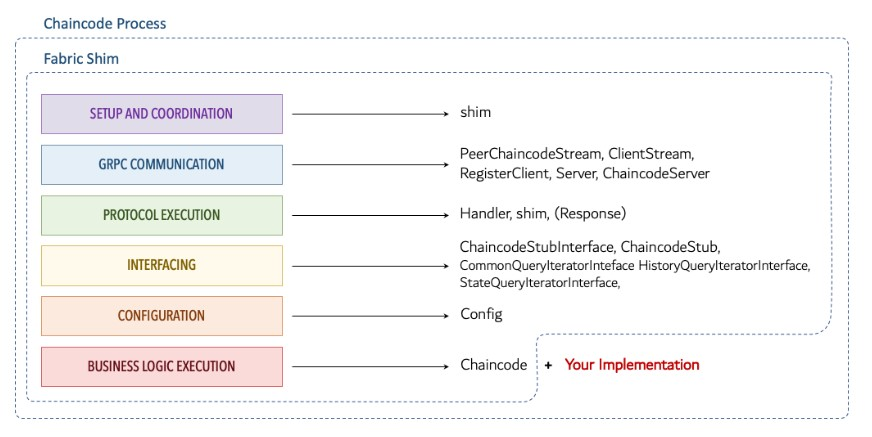
\includegraphics[width=\textwidth]{Images/chaincode_shim}
\caption{Componentes del chaincode shim}
\label{fig:chaincodeshim}
\end{figure}


\subsection*{Patrones de ejecución de Chaincode}

El \textit{shim} de Fabric admite dos modalidades de ejecución, que controlan el comportamiento de la conexión entre el \textit{chaincode} y el nodo \textit{peer}:

\begin{enumerate}
\item \textbf{Chaincode como cliente:} esta es la modalidad por defecto y la única utilizada en Hyperledger Fabric v1.4 [\cite{hlf-internals}]. Presenta el proceso chaincode como un cliente que inicia la conexión con el \textit{peer}.

\item \textbf{Chaincode como servidor:} A partir de la versión 2.0, Hyperledger Fabric admite la implementación de chaincode fuera de la blockchain [\cite{hlf-internals}]. De esta forma, el chaincode se ejecuta como un servidor independiente del \textit{peer}. En este escenario, no es necesario construir y lanzar el chaincode para cada \textit{peer}.
\end{enumerate}

\subsection*{Protocolo de interacción}
El protocolo de interacción se basa completamente en el intercambio de mensajes \textit{Protobuf} de tipo \texttt{ChaincodeMessage} entre el proceso chaincode y el \textit{peer}. La ventaja de usar \textit{Protobuf} es desacoplar la semántica de la implementación.

\begin{figure}[tbph]
\centering
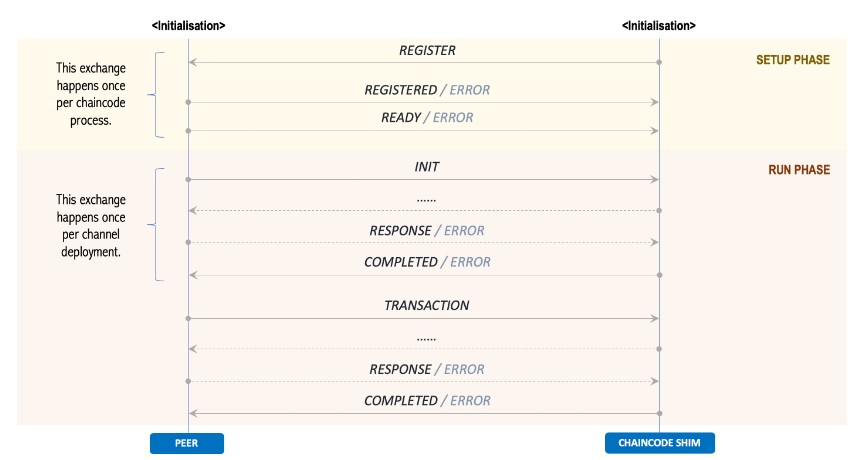
\includegraphics[width=\textwidth]{Images/interaction_protocol}
\caption{Interacción entre cliente y servidor gRPC}
\label{fig:interactionprotocol}
\end{figure}

La figura \ref{fig:interactionprotocol} proporciona una descripción general del protocolo de interacción de extremo a extremo. El ciclo de vida de la interacción se desarrolla en tres fases: inicialización, configuración y ejecución de la transacción (o fase de ejecución). En las siguientes secciones se proporcionarán más detalles para cada una de las fases.

\subsection*{Fase 1: Inicialización}
Durante la fase de inicialización, el \textit{peer} realiza una serie de operaciones:

\begin{enumerate}

\item Inicializa un objeto \texttt{ChaincodeSupport} que expone los servicios del \textit{chaincode} al nodo \textit{peer}.

\item Inicia un servidor gRPC de tipo \texttt{ChaincodeSupportServer} y registra el servicio \texttt{ChaincodeSupport} para habilitar la interacción con los procesos del \textit{chaincode}.

\item Inicia un servidor gRPC de tipo \texttt{EndorserServer}  para recibir propuestas de transacción para ser aprobadas.
\end{enumerate}

Por otro lado, el \textit{shim} carga el \textit{chaincode} invocando la función  \texttt{shim.Start(Chaincode)}, encargada de realizar las siguientes operaciones:

\begin{enumerate}
\item \textbf{Inicialización del cliente gRPC:} se utiliza para conectarse al \textit{peer} y configurar un flujo bidireccional para intercambiar instancias de \texttt{ChaincodeMessage}.

\item \textbf{Inicialización del \textit{handler}:} este componente se encarga de procesar todos los mensajes enviados por el \textit{peer} y ejecutar las operaciones asociadas.

\item \textbf{Inicialización del ciclo de procesamiento de mensajes:} este se utiliza para recibir los mensajes del \textit{peer} y enviarlos al \textit{handler} para su posterior procesamiento.
\end{enumerate}

Esta modalidad de inicialización admite el patrón \textbf{chaincode como  cliente}, donde el proceso \textit{chaincode} es un cliente para el \textit{peer}. El \textit{shim} también tiene la capacidad de inicializarse para admitir el patrón \textbf{chaincode como servidor}, donde los roles se invierten.

\subsection*{Fase 2: Configuración}
Antes de iniciar el ciclo para recibir de mensajes, el \textit{shim} envía un mensaje \texttt{REGISTER} a través del flujo bidireccional abierto con el \textit{peer}. Este mensaje contiene los detalles del \textit{chaincode} para registrarse codificado como \texttt{ChaincodeID}.
Al recibir el mensaje, el \textit{peer} valida la información asociada al \textit{chaincode} y crea una instancia de \textit{Handler} para manejar el intercambio de mensajes con el proceso del \textit{chaincode}. Luego, el \textit{peer} responde con un mensaje \texttt{REGISTERED} e inmediatamente después con un mensaje \texttt{READY}, lo que indica la finalización del proceso de configuración.

\subsection*{Fase 3: Ejecución de la transacción}
Una vez que se completa la fase de configuración, el \textit{chaincode} y el \textit{peer} están listos para ejecutar transacciones.

%A partir de este punto, la interacción es impulsada por el peer, como resultado de las operaciones que envían los clientes de la aplicación al peer. Por lo general, implican el despliegue del chaincode en un canal específico y la posterior invocación de transacciones en el contrato inteligente implementado.

Esta interacción se implementa en los siguientes pasos:

\begin{enumerate}
\item Como resultado del despliegue del \textit{chaincode}, el \textit{peer} envía un mensaje \texttt{INIT}. 

%El \textit{handler} inicializa un contexto de transacción para la simulación de la propuesta de transacción asociada a la inicialización y envía el mensaje a través de un flujo bidireccional.

\item Tras la recepción del mensaje \texttt{INIT}, el \textit{handler} crea una nueva instancia de \textit{ChaincodeStub}, que representa la interfaz para los servicios expuestos al contrato inteligente. Luego se invoca \texttt{Chaincode.Init()} pasando el \textit{stub} como argumento.

\item El \textit{chaincode} ejecuta la inicialización del contrato inteligente y el método \texttt{Init()} se completa con éxito o con un error. El primero hace que se envíe un mensaje \texttt{COMPLETED} al \textit{peer}, mientras que el segundo provoca un mensaje de \texttt{ERROR}.

\item Al recibir el mensaje, el \textit{peer} invoca el método \texttt{Handler.Notify()} en la instancia asociada al \textit{chaincode}. Este método cierra el contexto de transacción previamente abierto y hace que el método \texttt{Handler.Execute()} desbloquee y devuelva la respuesta obtenida por el \textit{chaincode}.

\end{enumerate}

Las invocaciones posteriores del mismo \textit{chaincode} en el mismo canal dan como resultado que el \textit{peer} envíe un mensaje \texttt{TRANSACTION}, que se maneja de la misma manera que se detalla para el mensaje \texttt{INIT}.







\chapter{Propuesta}\label{chapter:proposal}
En el presente capítulo se explica la solución al problema fundamental de este trabajo. Se propone la creación de una fabric-chaincode-api que permita la implementación de contratos inteligentes en el lenguaje $ C\sharp $.

La sección $ 2.1 $ aborda las herramientas que facilitan la conexión entre el chaincode y el nodo peer en el lenguaje $ C\sharp $.

En $ 2.2 $ se trata la solución al problema del procesamiento concurrente de transacciones.

En $ 2.3  $se explica la comunicación con el peer para las consultas al ledger.

\section{gRPC y \textit{protocol buffers}}

El chaincode se ejecuta en un entorno desacoplado al resto del nodo \textit{peer}. De esta forma, el \textit{peer} es independiente del lenguaje real en el que se implementa el chaincode. Para cumplir el propósito de este trabajo es necesario implementar el chaincode en $ C\sharp$, lenguaje distinto al del nodo peer (Go). En esta sección se explica gRPC [\cite{grpc-doc}], herramienta que permite la comunicación entre ambos. 

GRPC son las siglas que definen a un \textit{framework} desarrollado por Google sobre Llamada a Procedimiento Remoto (Remote Procedure Call, RPC por sus siglas en inglés). En gRPC, una aplicación cliente puede llamar directamente a un método en una aplicación servidor en una máquina diferente como si fuera un objeto local, lo que facilita la creación de aplicaciones y servicios distribuidos. 

Como en muchos sistemas RPC, gRPC se basa en la idea de definir un servicio, especificando los métodos que se pueden llamar de forma remota con sus parámetros y tipos de devolución. En el lado del servidor, se implementa una interfaz para manejar las llamadas de los clientes. En el lado del cliente, se tiene un \textit{stub} que proporciona los mismos métodos que el servidor.

La diferencia con otros frameworks RPC existentes es que gRPC usa \textit{protocol buffers} [\cite{protobuf-doc}] como lenguaje de definición de interfaz para la serialización y como formato de intercambio de mensajes en lugar de JSON/XML.

Los \textit{protocol buffers} proporcionan un mecanismo extensible, independiente del idioma y de la plataforma, para serializar datos estructurados de manera compatible con versiones anteriores y posteriores. Se pueden ampliar con nueva información sin invalidar los datos existentes ni requerir que se actualice el código.

\begin{figure}[tbph]
\centering
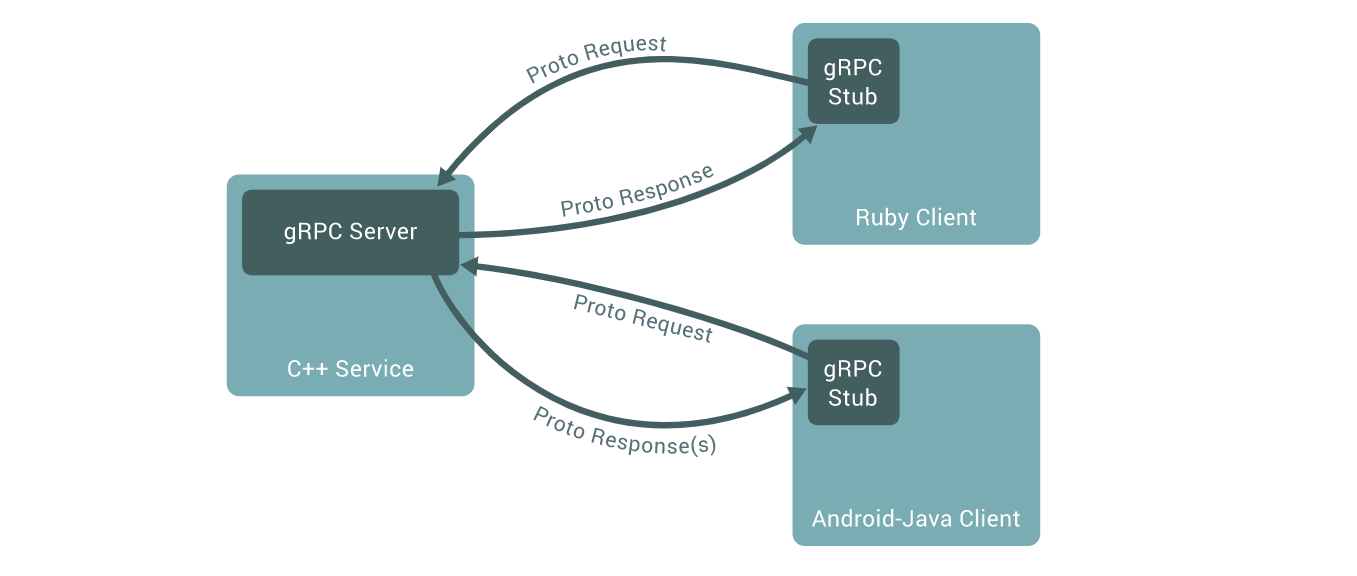
\includegraphics[width=\textwidth]{Images/grpc}
\caption{ Ejemplo de servidor C++ con clientes Ruby y Java.}
\label{fig:grpc}
\end{figure}

Los clientes y servidores de gRPC pueden ejecutarse y comunicarse entre sí en una variedad de entornos y pueden escribirse en cualquiera de los idiomas compatibles con gRPC. En la solución propuesta en este artículo se aprovecha dicha característica para comunicar al nodo \textit{peer} con el chaincode, escritos en Go y $ C\sharp$ respectivamente.

\section{fabric-protos-csharp}
Como se vio en el capítulo anterior, la interacción entre el chaincode y el nodo peer se establece mediante mensajes \textit{protobuf}. El servicio gRPC y las definiciones de \textit{protocol buffers} que se utilizan en Hyperledger Fabric se encuentran en el repositorio \textit{fabric-protos}, de dominio público. Se empleó la herramienta \texttt{protoc} para compilar estas definiciones al lenguaje C$\sharp$. De esa manera se crean las clases bases necesarias para interactuar con Fabric.

%\section{getChannelId}
%\section{getTxTimeStamp}
%\section{getCreator}
%\section{createCompositeKey}
%\section{splitCompositeKey}
%\section{getState}
%\section{putState}
%\section{deleteState}
\chapter{Experimentación y Resultados}\label{chapter:implementation}
En este capítulo se exponen los resultados, las ventajas, desventajas y comparaciones de usar la biblioteca \texttt{fabric-chaincode-csharp} con respecto a las implementadas en otros lenguajes.

\section{Ventajas del uso de $ C\sharp $ en Hyperledger Fabric}
La biblioteca propuesta permite la creación de contratos inteligentes en  $ C\sharp $. Como resultado, es posible aprovechar características propias del lenguaje para crear aplicaciones sólidas y duraderas sobre Hyperledger Fabric. Para respaldar esta afirmación se analizarán ejemplos de contratos inteligentes escritos en $ C\sharp $ que implementan la interfaz \texttt{IChaincode} propuesta en la biblioteca \texttt{fabric-chaincode-csharp}.



\begin{figure}[tbph]
\centering
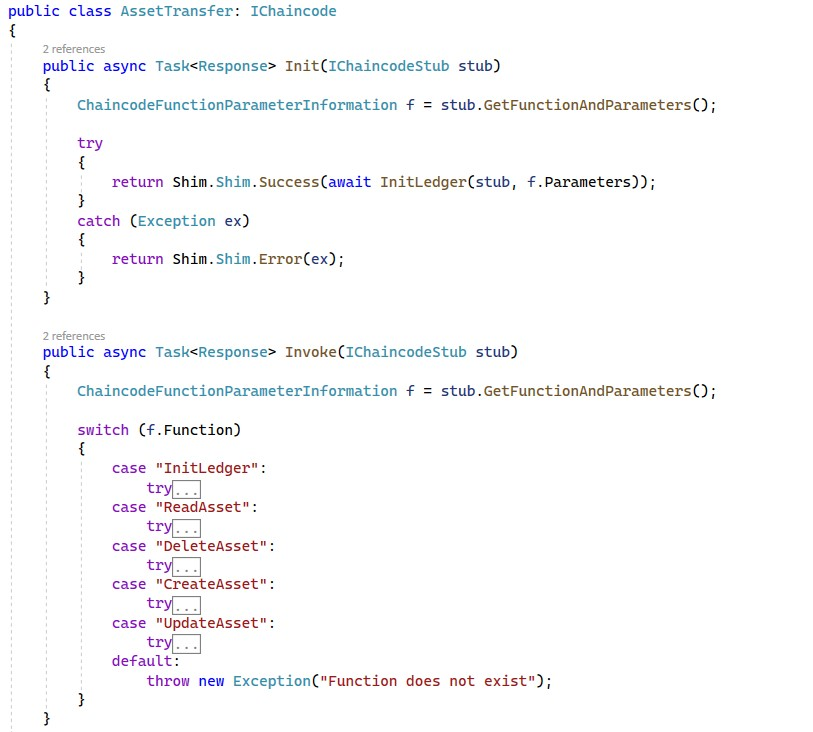
\includegraphics[width=\textwidth]{Images/assettransfer}
\caption{Contrato inteligente \texttt{AssetTransfer}}
\label{fig:assettransfer}
\end{figure}


La figura \ref{fig:assettransfer} muestra el contrato inteligente \texttt{AssetTransfer}, el cual aprovecha las características:

\begin{enumerate}

\item Interfaces. Se emplea la interfaz IChaincodeStub para agrupar las funcionalidades que permiten acceder a los servicios de invocación del ledger. La interfaz IChaincode provee al contrato los métodos que constituyen el punto de entrada para realizar propuestas de transacciones.

\item Soporte del lenguaje para operaciones asíncronas. Permite ejecutar de forma concurrente las funciones que necesitan interactuar con el peer para devolver un resultado, en este caso \texttt{InitLedger}, \texttt{ReadAsset}, \texttt{DeleteAsset}, \texttt{CreateAsset} y \texttt{UpdateAsset}. 

\item Genericidad. Se utiliza \texttt{Task<T>} en los métodos del contrato para representar una operación asíncrona que devuelve un valor de tipo \texttt{T}. Esto facilita la implementación de contratos, pues evita tener que crear una clase que soporte operaciones asíncronas por cada tipo que se quiera retornar.

%Las funciones del contrato que interactúan con el peer deben retornar Task para poder realizarse de forma concurrente.

%Se utiliza en el tipo \texttt{Task<Response>}. Usar un parámetro de tipo genérico, permite escribir una sola clase que otro código de cliente puede usar sin incurrir en el costo o el riesgo de las conversiones en tiempo de ejecución o las operaciones de \textit{boxing}.

\item Manejo de excepciones. Se utiliza la expresión \texttt{try/catch} para lidiar con errores durante la ejecución de una transacción. Permite escribir un código confiable, lo menos propenso a fallos posible.
\end{enumerate}

\section{Experimentación}

Para probar el correcto funcionamiento de la herramienta propuesta, se crearon numerosos contratos inteligentes. A continuación, se analizará un ejemplo.

A partir de la biblioteca propuesta el contrato inteligente \texttt{AssetTransfer} puede interactuar con la red \textit{blockchain} y realizar las operaciones: 

\begin{enumerate}
\item \texttt{CreateAsset}: Añade un elemento al \textit{ledger} a partir de la función del \textit{stub} \texttt{PutState(key, value)}.\\

\begin{lstlisting}[caption={Función \texttt{CreateAsset(...)}}]
public async Task<ByteString> CreateAsset(IChaincodeStub stub, Parameters parameters)
{

    parameters.AssertCount(2);
    string key = parameters[0];
    string value = parameters[1];


    var asset = new Asset(value);
    string jsonString = JsonSerializer.Serialize(asset);

    await stub.PutState(key, ByteString.CopyFromUtf8(jsonString));
    
    return ByteString.Empty;
}
\end{lstlisting}

\item \texttt{ReadAsset}: Devuelve un elemento del \textit{ledger} a partir de la función del \textit{stub} \texttt{GetState(key)}.\\

\begin{lstlisting}[caption={Función \texttt{ReadAsset(...)}}]
 public async Task<ByteString> ReadAsset(IChaincodeStub stub, Parameters parameters)
{
    string key = parameters[0];
    var asset =  await stub.GetState(key);
    if (asset == null || asset.Length <= 0) 
    	throw new Exception ("Asset {key} does not exist.");

    return asset;
}
\end{lstlisting}

\item \texttt{UpdateAsset}: Modifica un elemento del \textit{ledger} a partir de la función del \textit{stub}\texttt{ PutState(key)}.\\

\begin{lstlisting}[caption={Función \texttt{UpdateAsset(...)}}]
public async Task<ByteString> UpdateAsset(IChaincodeStub stub, Parameters parameters)
{
    string key = parameters[0];
    string value = parameters[1];

    var serializedJson = await stub.GetState(key);
    var asset = JsonSerializer.Deserialize<Asset>(serializedJson.ToStringUtf8());
    asset.Value = value;
    
    string jsonString = JsonSerializer.Serialize(asset);
    var updatedAsset = await stub.PutState(key, ByteString.CopyFromUtf8(jsonString));
    
    return ByteString.Empty;
}
\end{lstlisting}

\item \texttt{DeleteAsset}: Elimina un elemento del \textit{ledger} a partir de la función del \textit{stub} \texttt{DeleteState(key)}.\\

\begin{lstlisting}[caption={Función \texttt{DeleteAsset(...)}}]
public async Task<ByteString> DeleteAsset(IChaincodeStub stub, Parameters parameters)
{
    string key = parameters[0];
    await stub.DeleteState(key); 
    return ByteString.Empty;
}
\end{lstlisting}
\end{enumerate}

%Crear, Leer, Actualizar y Borrar, conocidas como operaciones CRUD por sus siglas en inglés.




%En este ejemplo se evidencia el manejo de excepciones y el soporte del lenguaje para operaciones asíncronas. El primero a través de la expresión try/catch y el segundo en el uso de las palabras clave async, await y Task. Sigue lo que se conoce como Patrón Asíncrono Basado en Tareas (TAP)  espera una operación que devuelva una Tarea o Task<T> dentro de un método asíncrono.


%C# tiene un modelo de programación asíncrona a nivel de lenguaje, que permite escribir fácilmente código asíncrono sin tener que hacer malabarismos con las devoluciones de llamada o ajustarse a una biblioteca que admita la asincronía. Sigue lo que se conoce como Patrón Asíncrono Basado en Tareas (TAP). 
%
%El modelo es bastante simple: espera una operación que devuelva una Tarea o Task<T> dentro de un método asíncrono.
%
%El núcleo de la programación asincrónica son los objetos Task y Task<T>, que modelan operaciones asincrónicas.
%
%La palabra clave async convierte un método en asíncrono, lo que le permite usar la palabra clave await en su cuerpo.
%
%Cuando se aplica la palabra clave await, suspende el método de llamada y devuelve el control a la persona que llama hasta que se completa la tarea esperada.




%$ C\sharp $ es un lenguaje orientado a objetos. Este paradigma de la programación fomenta la productividad en el desarrollo de \textit{software} mediante las propiedades: encapsulación, herencia y polimorfismo. La primera consiste en la posibilidad de una clase o estructura de especificar qué tan accesible es cada uno de sus miembros. La herencia es útil cuando se necesita agregar funcionalidad a un tipo existente. El polimorfismo permite que en tiempo de ejecución, los objetos de una clase derivada pueden tratarse como objetos de una clase base en lugares como parámetros de método.

%Otras facilidades que provee el lenguaje $ C\sharp $ incluyen:
%
%\begin{enumerate}
%\item Las expresiones \textit{lambda} admiten técnicas de programación funcional.
%
%\item  Admite tipos por referencia y por valor definidos por el usuario. 
%
%\item  Los tipos anulables protegen contra variables que no hacen referencia a objetos asignados.
%
%\item El manejo de excepciones proporciona un enfoque estructurado y extensible para la detección y recuperación de errores.
%
%\item El soporte de lenguaje para operaciones asíncronas proporciona sintaxis para construir sistemas distribuidos.
%\end{enumerate}

Si se compara con \texttt{fabric-chaincode-go} la biblioteca propuesta tiene como ventaja la capacidad de crear procesos concurrentes dentro de una misma transacción. Esto gracias a la implementación de la clase \texttt{MsgQueueHandler}, la cual maneja la interacción con el \textit{peer} a través de un diccionario que asocia a cada transacción una cola de mensajes. De esta forma, pueden existir varios hilos dentro del contexto de una misma transacción pues, el intercambio con el \textit{peer} se realiza de forma síncrona en el orden en que se añaden los mensajes en la cola.

%Aparte de las ventajas mencionadas, también existen limitaciones.
%La \texttt{fabric-chaincode-api} propuesta no implementa todas las funcionalidades que existen en el resto de bibliotecas. Por ejemplo, en Javascript/Typescript la \texttt{ChaincodeStubInterface} expone varios métodos que posibilita recibir una secuencia de datos del peer. Esta capacidad es útil pues permite, entre otras cosas, obtener un rango de llaves que cumplen con un determinado criterio o la recuperación de los cambios históricos realizados en el valor asociado a una llave.



%\colorbox{lightgray}{PENDIENTE: Insertar código}
%
%\section{Recomendaciones}



%La implementación de esta capacidad se basa en iteradores. Se definen tres tipos diferentes:
%
%CommonIteratorInterface: define las operaciones comunes de todos los tipos de iteradores.
%
%StateQueryIteratorInterface: especializa la interfaz del iterador base para iterar sobre una colección de claves en el ledger.
%
%HistoryQueryIteratorInterface: esta interfaz especializa la interfaz del iterador base para iterar sobre el historial de cambios de una llave.






\backmatter

\begin{conclusions}
%En el presente trabajo se realizó un resumen de los conceptos principales de Hyperledger Fabric. Se hizo énfasis en las características de diseño que hacen posible la programación de contratos inteligentes en lenguajes de propósito general.

En el presente trabajo se llevó a cabo un estudio de las APIs existentes para Hyperledger Fabric que permiten escribir contratos inteligentes en otros lenguajes de programación. Se expusieron detalles del diseño e implementación de la biblioteca \texttt{fabric-chaincode-api} propuesta y finalmente se muestran los resultados obtenidos mediante ejemplos de contratos inteligentes programados en $ C \sharp $. Estos elementos contribuyeron al cumplimiento del objetivo general de este trabajo, el cual consiste en poder integrar la lógica de los contratos inteligentes programados en $ C \sharp $ dentro de la arquitectura de una \textit{blockchain} Hyperledger Fabric.

En la \texttt{fabric-chaincode-api} propuesta quedan pendientes de implementación las funciones que permiten realizar consultas enriquecidas, trabajar con datos privados y lanzar eventos a nivel de \textit{chaincode}. Esto limita las aplicaciones que utilicen esta biblioteca a trabajar solamente con las operaciones: Crear, Leer, Actualizar y Eliminar. Dicho esto, las áreas en las que orientar el futuro de \texttt{fabric-chaincode-csharp} son:
    
\begin{enumerate}
\item Extender las funcionalidades expuestas en el \texttt{ChaincodeStub}.
\item Diseño e implementación de la biblioteca de alto nivel\\ \texttt{fabric-contract-csharp}.
\end{enumerate}

\end{conclusions}
%Por ejemplo, en Javascript/Typescript la \texttt{ChaincodeStubInterface} expone varios métodos que posibilita recibir una secuencia de datos del peer. Esta capacidad es útil pues permite, entre otras cosas, obtener un rango de llaves que cumplen con un determinado criterio o la recuperación de los cambios históricos realizados en el valor asociado a una llave.
%\begin{recomendations}
%    
%\end{recomendations}

\printbibliography[heading=bibintoc]

\end{document}